% fuentes de esta seccion
% https://www.sewio.net/uwb-technology/two-way-ranging/

\chapter{Marco teórico}

Todo proyecto robótico tiene por objeto crear un sistema complejo, cuyo desarrollo requiere conocimientos interdisciplinarios. El robot se coloca, de hecho, en la frontera entre la mecánica, la electrónica, el automóvil y la informática, lo que dentro de la industria 4.0 se denomina un sistema ciberfísico. Con todo esto podemos decir que nuestro robot debe contar con, al menos, las siguientes características:

\begin{itemize}
    \item Poseer 4 ruedas omnidireccionales controladas.
    \item Poder coexistir en el mismo espacio con otros robots.
    \item Determinar su posición en todo momento.
    \item Poder capturar imágenes con una cámara.
\end{itemize}

Se llevarán a cabo análisis de los puntos mencionados para conocer qué alternativas existen para abordar el proyecto y qué tópicos necesitamos conocer para llevar a cabo el desarrollo.

\section{Estado del arte}

La tecnología robótica se encuentra en plena fase de crecimiento, y por lo tanto, es previsible una presencia cada vez mayor de los robots, tanto en el sector industrial y de servicios, como en el sector doméstico. Como ha ocurrido en la informática, el desarrollo de robots se hace cada vez más accesible y por consiguiente sus capacidades tienden cada vez mayores gracias al aporte de una comunidad en auge. Este aumento en el interés de las personas sobre esta área, plantea ciertos desafíos, no solo en los aspectos tecnológicos, sino, también desde el punto de vista cultural y ético.

En la última mitad del siglo pasado el foco estaba puesto sobre todo en el campo de la robótica para impulsar el desarrollo de la producción a gran escala. Hoy se ha logrado gracias a ello un nivel tal de tecnología que el estudio y la realización de robots flexibles capaces de adaptarse a diferentes propósitos a diferentes entornos de trabajo ya no es una utopía. Desde el año dos mil, la investigación en el campo robótico también se dirige hacia el diseño de robots dedicados a la exploración del medio ambiente y de los llamados "robots de servicio".

Si hacemos foco en lo que respecta a los robots exploradores móviles, los mayores avances tecnológicos se dan en la exploración de otros planetas. Actualmente los científicos están enfocados en el planeta Marte así como lo fue en su momento la superficie Lunar. Los primeros desarrollos de este tipo de vehículos no tripulados surgen principalmente durante la carrera espacial entre USA y la URSS en la década del 60/70, donde los más conocidos, exceptuando los exploradores lunares han sido los siguientes:

Mars3 enviado en 1971 por la URSS el cual funcionó sobre la superficie marciana durante unos escasos 20 segundos.

\begin{figure}[H]
    \centering
    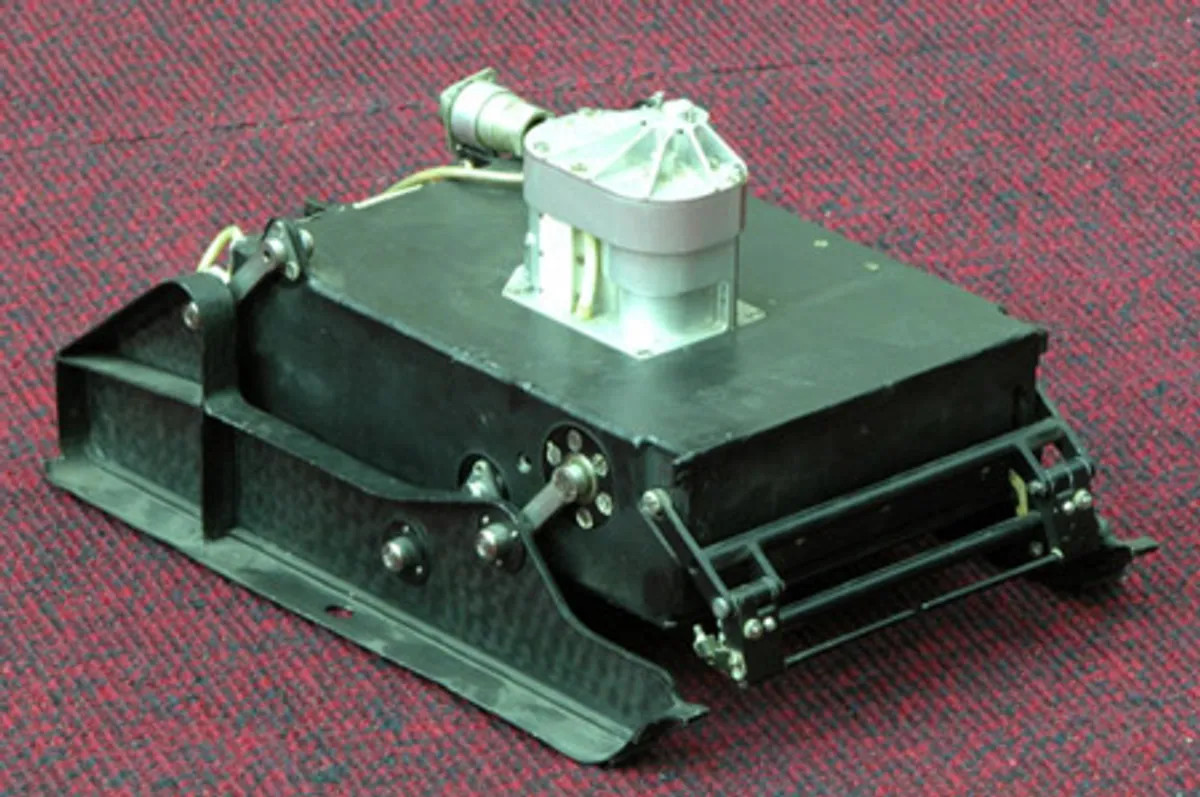
\includegraphics[width=0.5\linewidth]{images/mars3.jpg}
    \caption{Robot Mars3}
    \label{fig:mars3}
\end{figure}

En 2003, la NASA envió dos vehículos idénticos de 174 kilogramos con seis ruedas y paneles solares para recorrer parte de la superficie marciana, el Spirit y el Opportunity. El primero transmitió datos que hacen pensar que en el pasado existió agua líquida en Marte, hasta que se atasco y dejó de funcionar. El Opportunity todavía está operativo y ostenta el récord de distancia recorrida en otro planeta, con más de 42,6 kilómetros hasta el momento.

\begin{figure}[H]
    \centering
    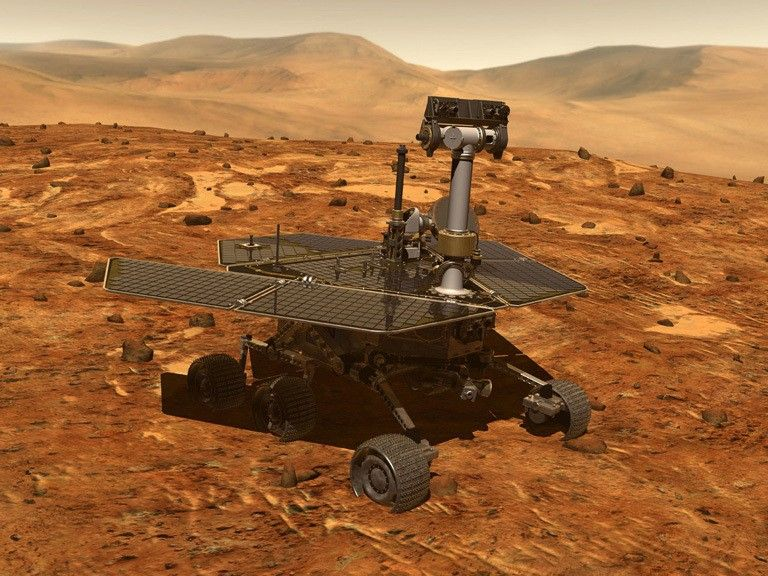
\includegraphics[width=0.5\linewidth]{images/opportunity-3d-model.jpg}
    \caption{Robot Opportunity}
    \label{fig:robot_opportunity}
\end{figure}

En 2011 la NASA envió a Marte el Curiosity, el vehículo más pesado (899 kilogramos) que nunca ha llegado a ese planeta. Aún está operativo y ha aportado las primeras evidencias de moléculas orgánicas en el planeta rojo.

\begin{figure}[H]
    \centering
    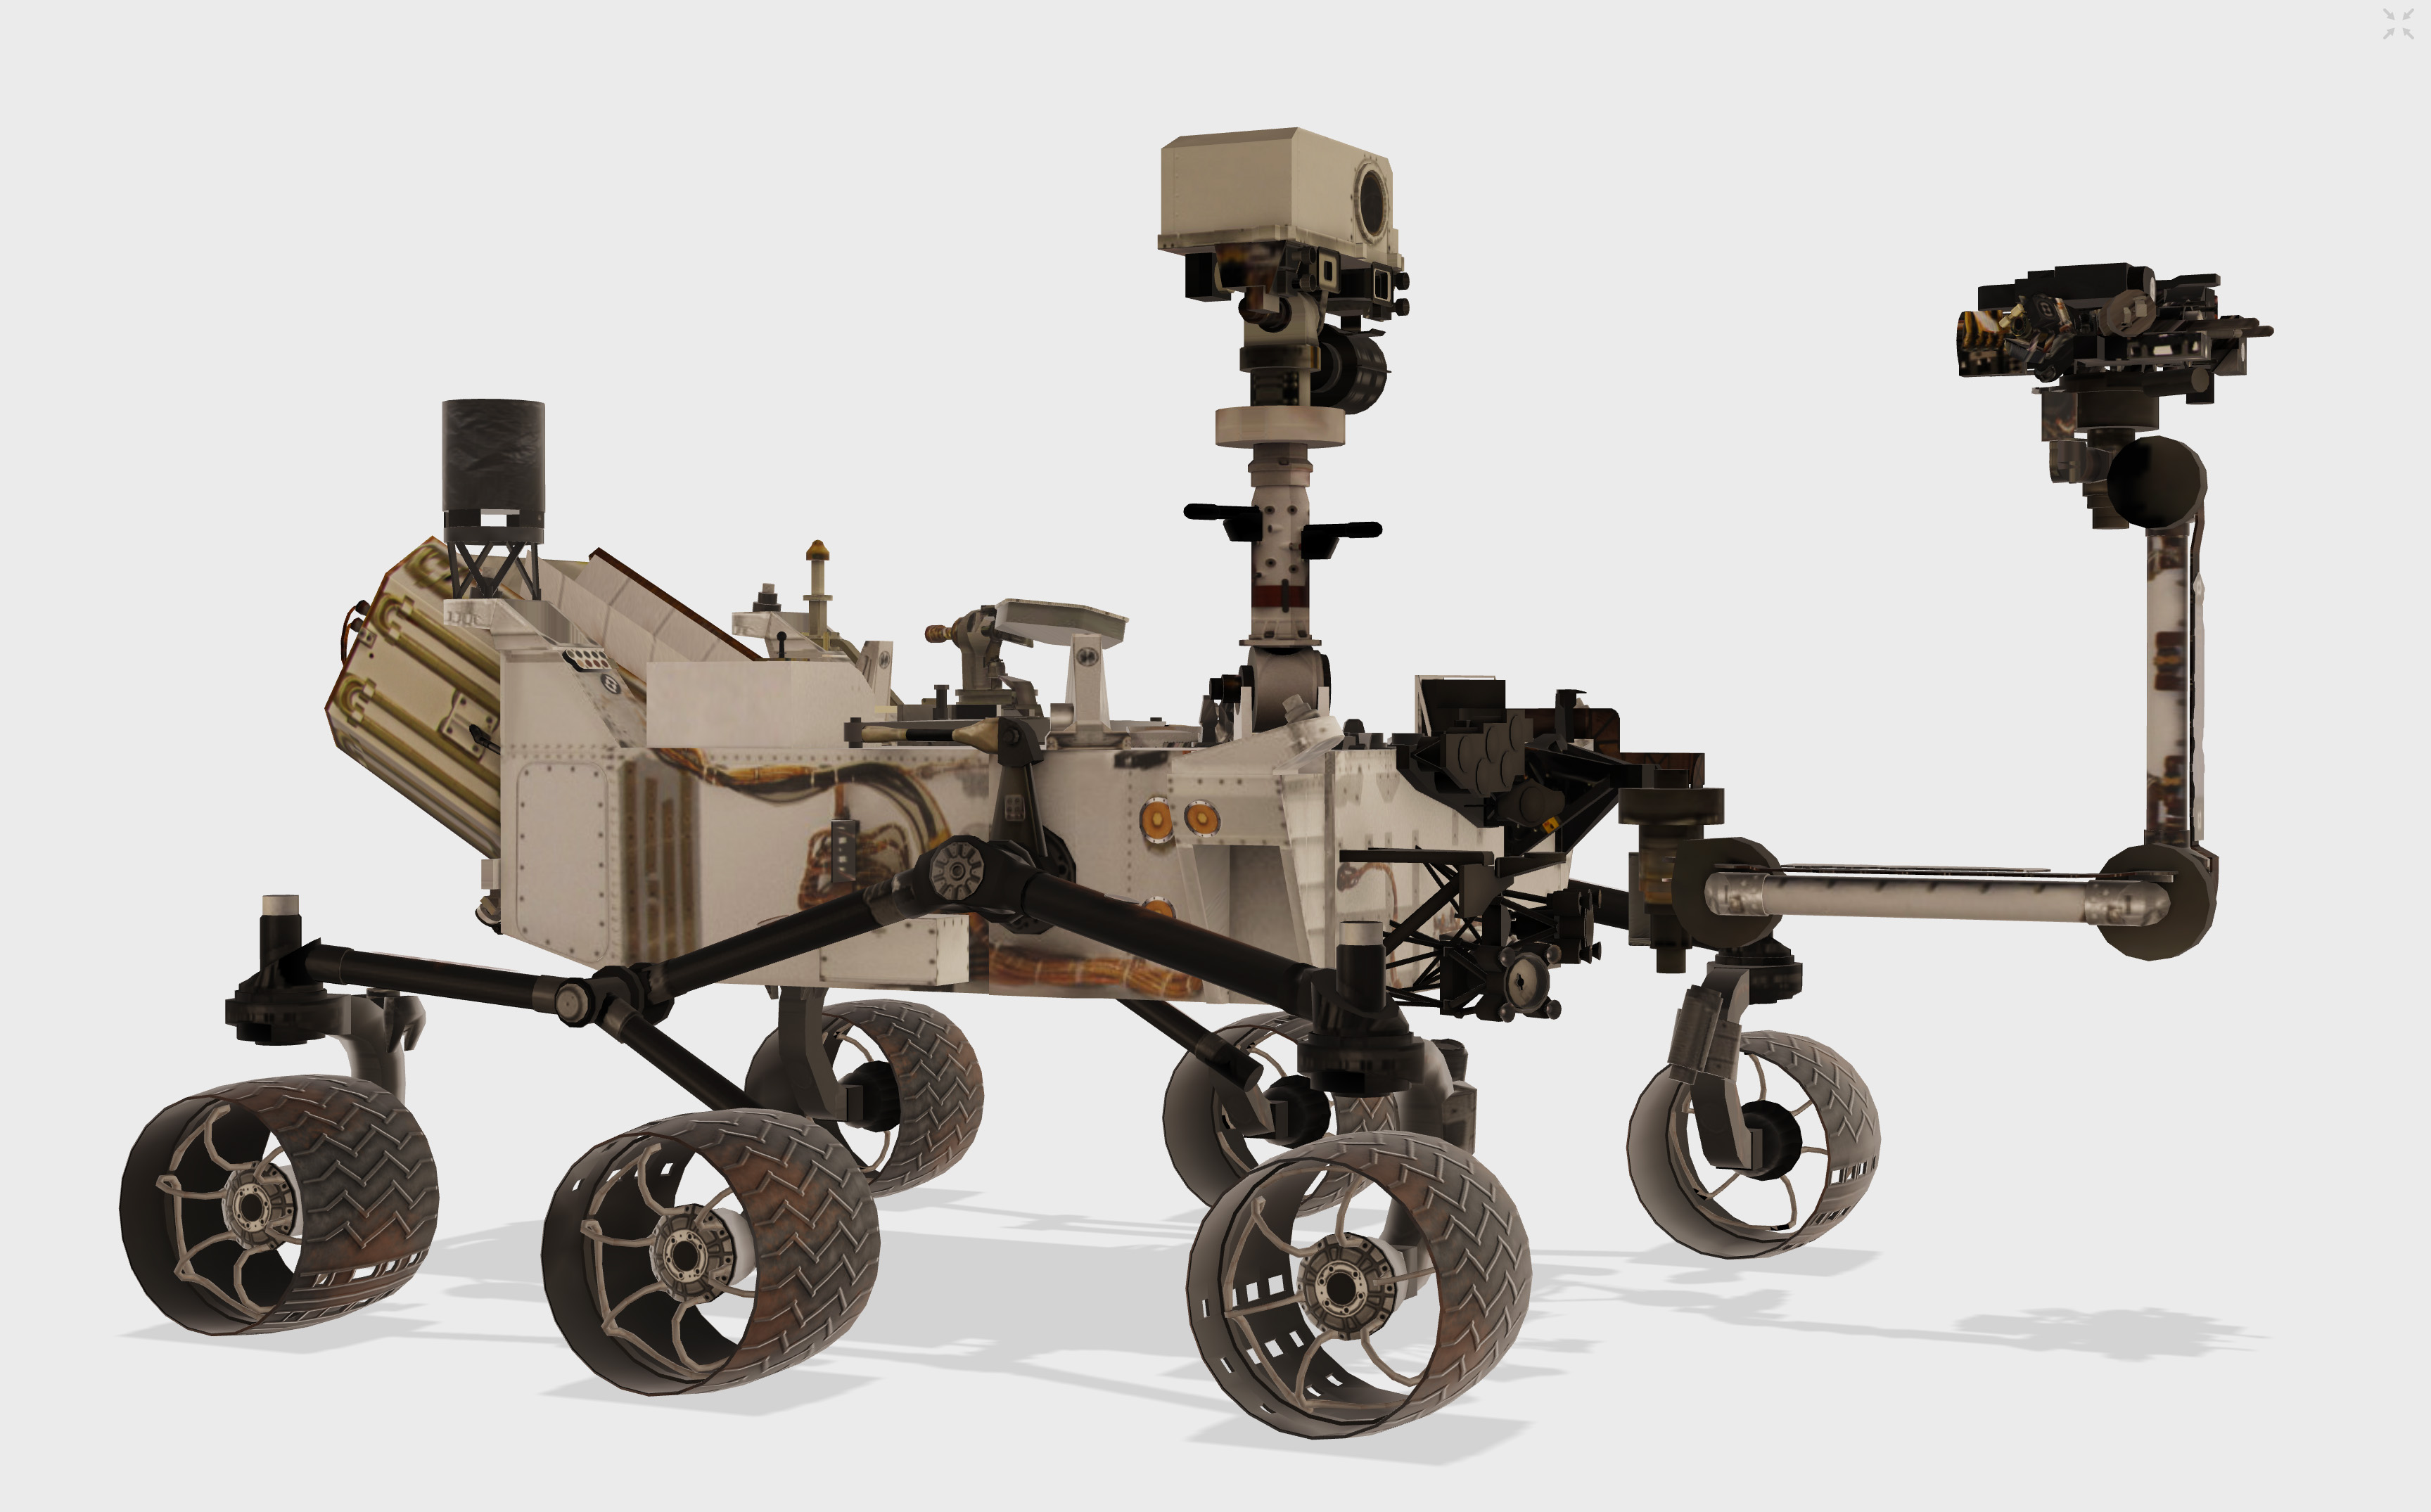
\includegraphics[width=0.5\linewidth]{images/curiosity-3d-model.jpg}
    \caption{Robot Curiosity}
    \label{fig:robot_curiosity}
\end{figure}

El 14 de marzo de 2016 la ESA y la Roscosmos enviaron a Marte la misión ExoMars, la primera de dos misiones que buscan analizar la atmósfera y colocar en su superficie dos vehículos, el segundo (2018) capaz de excavar dos metros por debajo de la superficie.

\begin{figure}[H]
    \centering
    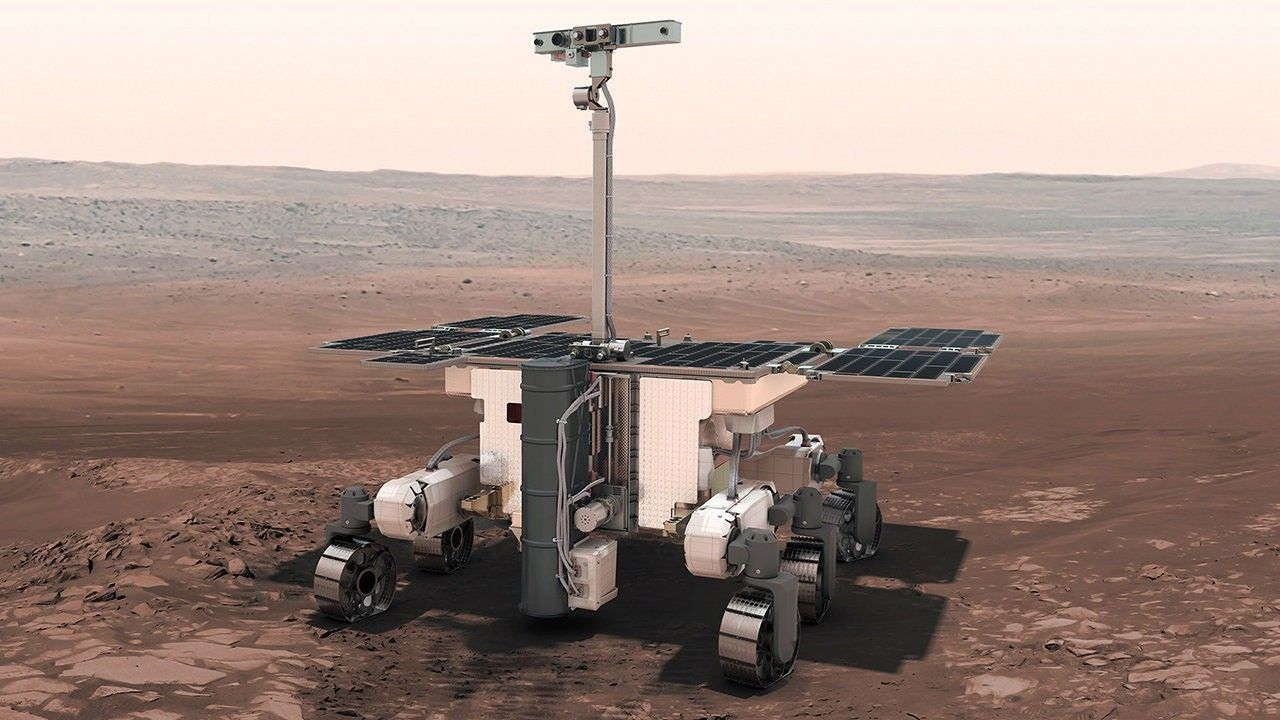
\includegraphics[width=0.5\linewidth]{images/Exomars_Rover.jpg}
    \caption{Robot ExoMars Rover}
    \label{fig:robot_exomarsrover}
\end{figure}

Por otra parte, tenemos a la robótica de servicio que es útil en el campo de la robótica médica, para la asistencia en rehabilitación y cirugía, así como en el campo doméstico para realizar tareas de limpieza y vigilancia.

La robótica móvil para estos sectores se ha convertido en una "herramienta de trabajo" importante y cada vez adquiere mayor protagonismo.

En los últimos años, mientras que la investigación de punta se enfoca en el diseño de robots para la exploración de Marte, en virtud de las tecnologías desarrolladas para tal fin, se hicieron los primeros robots para uso civil. Algunos de ellos, gracias a su pequeño tamaño y bajo costo de producción, gozan de cierto éxito comercial. Podemos mencionar de ejemplos al robot Roomba, hecho para la limpieza y lavado de pisos, una tarea que podría considerarse sencilla pero que implica un intenso trabajo computacional.

Sea cual sea el ámbito de aplicación, el diseño de robots móviles de pequeño tamaño y bajo costo de producción, pero, equipados con lógica de control avanzada, ha demostrado ser una gran utilidad para el hombre.

\section{Codiseño hardware-software}

El codiseño hardware-software es un enfoque metodológico que busca optimizar el rendimiento, la eficiencia y la funcionalidad de un sistema mediante la integración y colaboración estrecha entre el diseño del software y el hardware desde las etapas iniciales del desarrollo. En el contexto de un robot omnidireccional, la arquitectura de alto nivel debe ser cuidadosamente planificada para garantizar que ambos componentes trabajen de manera sinérgica, maximizando las capacidades del sistema y minimizando sus limitaciones. En nuestro caso se trata de un cyberphysical system dado que combina elementos de hardware, software y conectividad.

A continuación, se presentan las consideraciones clave y los tópicos más relevantes en el proceso de codiseño.

\subsection{Consideraciones clave}
El desarrollo de un sistema robótico eficiente y funcional requiere una definición clara y precisa de los requerimientos tanto funcionales como no funcionales. Al definirlos podemos encontrar aspectos como la precisión en la navegación, la capacidad de procesamiento en tiempo real, el consumo energético y la escalabilidad del diseño. Además, es esencial considerar las restricciones técnicas vinculadas al tamaño, el peso, el costo y la disponibilidad de los componentes, ya que estos factores tienen un impacto directo en las decisiones de diseño del sistema.

Un robot omnidireccional necesita realizar múltiples tareas de manera simultánea, como el procesamiento de datos sensoriales, la planificación de trayectorias y el control de los actuadores. Por ello resulta indispensable evaluar qué partes del sistema pueden ejecutarse de forma concurrente y distribuir las tareas entre el hardware y el software de modo eficiente.

La interacción entre el software y el hardware debe estar diseñada para garantizar una comunicación fluida y eficiente, minimizando los cuellos de botella que puedan limitar el rendimiento del sistema. Este aspecto incluye la selección adecuada de protocolos de comunicación, como SPI, I2C o Ethernet, así como la optimización del flujo de datos con el objetivo de reducir la latencia y mejorar la capacidad de respuesta general. \cite{lee2017introduction}

El uso equilibrado de los recursos hardware, como memoria, capacidad de cómputo y energía, con las demandas del software es otro factor esencial para optimizar el rendimiento del sistema. Se pueden implementar técnicas de optimización, como la compresión de datos o la reducción en la frecuencia de muestreo, siempre y cuando no se comprometa la funcionalidad del robot.

La arquitectura del sistema se diseña bajo principios de modularidad y escalabilidad, permitiendo la incorporación de nuevas funcionalidades o actualizaciones de componentes sin que se vea afectado el diseño global. Esta aproximación facilita la adaptabilidad del sistema a las necesidades futuras y contribuye a mitigar los costos asociados con la obsolescencia tecnológica.

Además, para garantizar la estabilidad y confiabilidad del sistema, es fundamental incorporar mecanismos de redundancia y recuperación ante fallos tanto en el hardware como en el software. La implementación de sistemas de monitoreo en tiempo real permite detectar errores de manera proactiva y corregirlos antes de que impacten la funcionalidad general del robot, asegurando así su robustez y tolerancia ante posibles fallos.


\subsection{Análisis de elementos necesarios}

Se analizan los elementos esenciales con los que debemos contar para así lograr la realización del proyecto. Estos elementos constituyen la base del proyecto, por lo que las decisiones tomadas al comienzo pueden repercutir en una etapa avanzada del mismo.


\subsubsection{Plataforma de hardware}

La selección de la plataforma hardware constituye un aspecto fundamental en el diseño de un sistema robótico, ya que debe equilibrar aspectos como la potencia de cálculo, el consumo energético y el costo. Entre las opciones disponibles, se encuentran los microcontroladores, como los basados en ARM Cortex u otros tales como Raspberry Pi, NVIDIA Jetson y las FPGAs. Están destinados a contener la lógica de control, monitoreo y comunicación inalámbrica. La plataforma elegida debe ser capaz de realizar operaciones en tiempo real.

También resulta crucial integrar componentes como sensores y actuadores que interactúen con el entorno. Los actuadores son los dispositivos encargados de interactuar con el medio en el que el robot se dispone y los sensores son los encargados de tomar muestras de magnitudes físicas de interés, como velocidad y distancia. \cite{lee2017introduction}

Dado que el robot debe operar con baterías y éstas son de capacidad limitada, la gestión de energía se convierte en un factor crítico. Optimizar el consumo energético requiere técnicas como el escalado dinámico de frecuencia o la hibernación de componentes no utilizados. También es recomendable incluir baterías de alta capacidad o sistemas de recarga automática para extender la autonomía del robot y mejorar su sostenibilidad operativa.


\subsubsection{Plataforma de software}
En cuanto a la arquitectura de procesamiento, es necesario definir si el diseño será centralizado, con un único procesador, o distribuido, utilizando múltiples procesadores o núcleos. Para sistemas complejos, como los robots omnidireccionales, una arquitectura distribuida suele ser preferible, ya que permite asignar tareas específicas a unidades de procesamiento dedicadas. Esta estrategia no solo optimiza el rendimiento del sistema, sino que también incrementa su eficiencia operativa en escenarios exigentes.

El desarrollo de software debe realizarse utilizando sistemas operativos en tiempo real o frameworks especializados, como ROS (Robot Operating System) o FreeRTOS, que permiten una gestión eficiente de tareas y recursos. A su vez, es fundamental implementar algoritmos optimizados para funciones clave como la navegación, la localización y el control, con el objetivo de garantizar un desempeño confiable en condiciones reales.

Debe señalarse además que son necesarios mecanismos lógicos de control para modelar todo el sistema junto con sus reglas. Para esto existen herramientas como Redes de Petri, que nos permiten modelar sistemas complejos con elementos sencillos.

Del mismo modo, la plataforma de software debe proveer al usuario de una interfaz interactiva donde pueda ejecutar órdenes y monitorear el estado de los robots en todo momento.


\subsubsection{Comunicación y sincronización}
El diseño de la comunicación y sincronización entre los distintos módulos del robot es esencial para garantizar un funcionamiento fluido y coordinado. Es indispensable implementar un sistema de comunicación eficiente que conecte sensores, actuadores y la unidad de control, además de mecanismos de sincronización que aseguren que las tareas se ejecuten en el orden y momento correctos, optimizando así el rendimiento global del sistema. \cite{lee2017introduction}

Al mismo tiempo, la latencia resulta crítica en aplicaciones robóticas. Una baja latencia asegura que el robot pueda reaccionar de manera inmediata a cambios en su entorno, como la aparición de obstáculos o la necesidad de ajustar su trayectoria. Esto es particularmente importante en entornos dinámicos, donde los retrasos en la toma de decisiones pueden resultar en colisiones o fallos en la navegación.


\subsubsection{Localización en tiempo real}

Para lograr que el robot navegue de modo autónomo, debemos utilizar los sensores y algoritmos avanzados de control, navegación y aprendizaje automático. Un sistema de cómputo potente permite implementar técnicas como el Filtro de Kalman para la estimación de la posición, algoritmos de planificación de rutas y sistemas de control predictivo, lo que mejora la precisión y eficiencia del robot. Todo esto permite la implementación de navegación autónoma, junto con la detección y evitación de obstáculos en tiempo real, además de integrar tareas de reconocimiento y aprendizaje.

Para justificar esto, debemos pensar que un robot omnidireccional dependerá de una gran cantidad de datos provenientes de sensores (cámaras, sensores de proximidad, giroscopios, etc.) para navegar y evitar obstáculos. Estos datos deben ser procesados en tiempo real para tomar decisiones rápidas y precisas, por lo cual un sistema de cómputo con alta capacidad de cálculo permite realizar operaciones complejas, como la fusión de datos sensoriales, la ejecución de algoritmos de localización y mapeo (SLAM, Simultaneous Localization and Mapping), y la planificación de trayectorias, de manera eficiente y sin retrasos. Esto implica la necesidad de procesamiento de datos en tiempo real. \cite{sariffpathplan}

En las subsiguientes secciones de este capítulo se profundiza sobre los distintos aspectos que nos son necesarios para la realización del proyecto.


\section{Movimiento y posicionamiento en interiores}

El control del movimiento y posicionamiento requiere procedimientos robustos que integren estrategias de planificación y ejecución en tiempo real.

Para que el robot se mueva por medio de sus ruedas, se utilizan controladores PID (Proporcional, Integral y Derivativo), los cuales ajustan dinámicamente las velocidades de las ruedas. Por otro lado, los sistemas más avanzados pueden integrar estrategias de Control Predictivo por Modelo (MPC), optimizando la trayectoria del robot mediante predicciones basadas en el modelo cinemático. Adicionalmente, el robot debe incorporar sensores para la retroalimentación del movimiento, como encoders en las ruedas y acelerómetros. Esta información es utilizada para ajustar y corregir el control en tiempo real.

Los algoritmos de control, como los basados en PID (Proporcional, Integral y Derivativo) o MPC (Control Predictivo por Modelo), permiten ajustar las velocidades y trayectorias del robot de manera precisa para evitar colisiones y garantizar estabilidad. Además, la navegación en interiores puede beneficiarse de técnicas como la SLAM (Simultaneous Localization and Mapping), que combina la localización con la construcción de mapas del entorno, ofreciendo una representación dinámica y actualizada. Cabe destacar la existencia de estimadores de estado genéricos como ser Filtro de Kalman, que permite la fusión de datos de múltiples sensores.

En la actualidad, los sistemas de posicionamiento en interiores (IPS, por sus siglas en inglés) se han convertido en una herramienta esencial en la navegación en espacios cerrados. La implementación de estas tecnologías puede lograrse mediante el uso de balizas de radiofrecuencia (Bluetooth, Wi-Fi, banda ultra ancha UWB), ultrasonido, etiquetas RFID y comunicaciones por luz visible (VLC, por sus siglas en inglés). \cite{nuaimisurveyindoorpositioning}

A pesar de los avances logrados, el posicionamiento asistido por GPS en interiores presenta limitaciones significativas debido a la gran pérdida de trayectoria provocada por las paredes de los edificios. Este debilitamiento de la señal lo convierte en una opción poco viable en comparación con otras tecnologías más especializadas.

Por otro lado, el uso de ultrasonido presenta problemas derivados de la alta atenuación en el aire, lo que dificulta su aplicación en eventos que requieran un amplio alcance. Otros métodos de posicionamiento, como infrarrojos, Zigbee y Bluetooth, aunque prometedores, pueden ser vulnerables a fluctuaciones en las fuentes de señal. No obstante, esta limitación podría mitigarse a través de soluciones como la implementación de una granja de antenas para garantizar una señal estable. En términos de precisión, las tecnologías tradicionales como Wi-Fi, Bluetooth y RFID activo proporcionan una precisión que generalmente varía en el rango de varios metros.

En cuanto a las comunicaciones de luz visible (VLC), se destacan por su enfoque innovador al detectar luz mediante fotodetectores. El uso de un único detector permite realizar una lateralización circular, mientras que la implementación de dos detectores habilita un posicionamiento diferencial. Este último método ha demostrado un mejor desempeño y una mayor reducción en el margen de error, consolidándose como una solución prometedora para futuros desarrollos tecnológicos en el ámbito del posicionamiento en interiores.

Cambien podemos mencionar los seguidores de línea, que representan un ejemplo simplificado de navegación basada en detección. Se emplean sensores para identificar y seguir líneas o patrones, que actúan como guías para el control del movimiento y la localización en entornos estructurados.

A continuación se detalla una tabla comparativa sobre las diferentes alternativas para posicionamiento en interiores, entre ellos, los distintos sistemas de localización en tiempo real que existen, también conocidos como RTLS \cite{alammarsurveyindoor}.

\begin{figure}[H]
    \centering
    \hspace*{-1.0cm}
    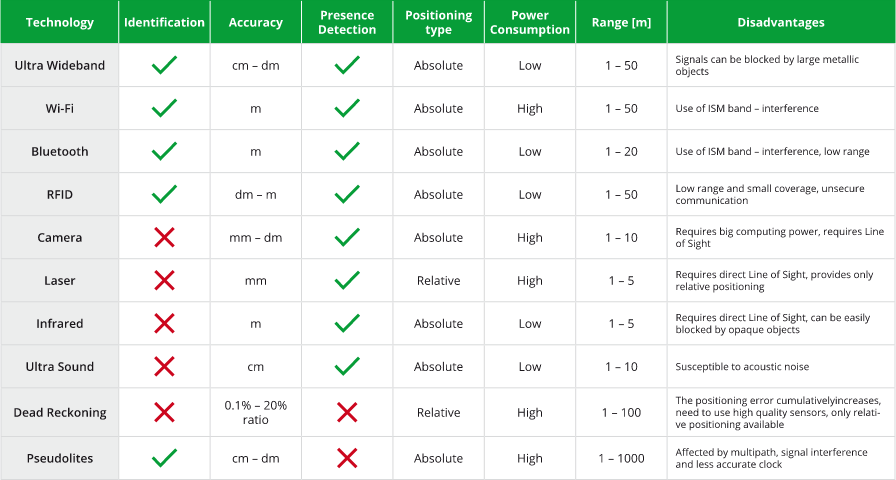
\includegraphics[width=1.1\linewidth]{mt_RTLS_comparacion}
    \caption{Tabla comparativa entre métodos de posicionamiento en interiores extraída de \textit{sewio.net} \cite{sewiortls}}
    \label{fig:compmetposindor}
\end{figure}


\subsection{Filtro de Kalman}

El filtro de Kalman constituye una herramienta esencial en la robótica para la estimación del estado de un sistema dinámico en entornos sujetos a incertidumbre y ruido en las mediciones. En el caso de robots omnidireccionales, su aplicación es particularmente útil para determinar la posición de un objeto en tiempo real mediante la integración de datos provenientes de múltiples sensores. Este proceso permite superar las limitaciones impuestas por el ruido inherente y las diferencias en las frecuencias de muestreo de los sensores.

El funcionamiento del filtro de Kalman se fundamenta en dos etapas principales: la predicción y la actualización. En la fase de predicción, se estima el estado del sistema y su incertidumbre utilizando modelos cinemáticos que describen el movimiento del objeto. En la etapa de actualización, las observaciones obtenidas de los sensores se incorporan para ajustar la estimación, ponderando cada medición según su nivel de precisión. Este enfoque posibilita la integración eficaz de entradas provenientes de sensores como cámaras, acelerómetros, encoders, entre otros, incluso cuando las frecuencias de muestreo difieren entre sí. \cite{nuaimisurveyindoorpositioning}


\subsection{Detección y medición de QR}

La detección y utilización de códigos QR en la robótica interior han demostrado ser una solución económica y eficiente para la navegación y localización del robot. Estos códigos, colocados en paredes y áreas visibles, pueden almacenar información relevante sobre el entorno, como la sección o ubicación específica dentro del espacio. Además, su bajo costo de producción los hace ideales para proyectos de robótica en interiores. \cite{tzafestas2013introduction}

La lectura de los códigos QR se realiza mediante cámaras integradas en el robot. Estas cámaras capturan imágenes del código y, utilizando técnicas de procesamiento de imagen, decodifican la información almacenada. Además, se puede estimar la distancia entre el robot y el código QR con un nivel razonable de precisión, aprovechando el tamaño conocido del código y las características del encuadre de la cámara. Este cálculo, basado en principios de geometría proyectiva, permite al robot ajustar su posición y orientar sus movimientos en función de los datos obtenidos.


\section{Redes de Petri}

Una red de Petri es un modelo gráfico, formal y abstraco para la representación de sistemas distribuidos y el análisis del flujo de información. Este modelo facilita la comprensión sobre la estructura y el comportamiento dinámico y estático del sistema modelado. Las redes de Petri son de utilidad principalmente en el diseño de sistemas de hardware y software para especificación, simulación y diseño de diversos problemas de ingeniería, especialmente útiles para representar procesos concurrentes, asó como procesos donde puedan existir restricciones en cuanto a la simultaneidad, la precedencia o la frecuencia de eventos concurrentes.\\

Las redes de Petri están fuertemente asociadas a la teoría de grafos, ya que las mismas pueden representarse como un grafo dirigido bipartito compuesto por cuatro elementos:

\begin{itemize}
    \item Plazas: representan los estados del sistema. Estas son variables de estado que pueden tomar valores enteros.
    \item Tokens: figuran como puntos dentro de las plazas. Estos representan el valor específico de una condición o estado y generalmente se traducen a la presencia o ausencia de algún recurso del sistema.
    \item Transiciones: representan el conjunto de sucesos cuya ocurrencia produce la modificación de los estados (y en consecuencia del estado global) del sistema.
    \item Arcos: indican las interconexiones entre las plazas y las transiciones, estableciendo el flujo de tokens que sgieu el sentida de la flecha.
\end{itemize}

Una vez definidos sus componentes, se puede decir que una red de Petri es un grafo dirigido con dos tipos de nodos: plazas y transiciones. Estos nodos están vinculados por arcos, los cuales sólo puede conectar una plaza con una transición o viceversa. Por otro lado, una red de Petri puede ser descrita mediante dos componentes:

\begin{enumerate}
    \item Una estructura de red
    \item Un marcado inicial
\end{enumerate}

La estructura de red hace referencia a la red en sí, mientras que el marcador inicial sólo representa el estado inicial del sistema (denominado estado idle), es decir, sin que ninguna transición haya sido disparada. Un ejemplo simple de una red de Petri marcada se muestra en la Figura \ref{fig:rdp_marcada}. Este será utilizado en las secciones siguientes para ilustrar operaciones y/o propiedades de las redes de Petri.

\begin{figure}[H]
    \centering
    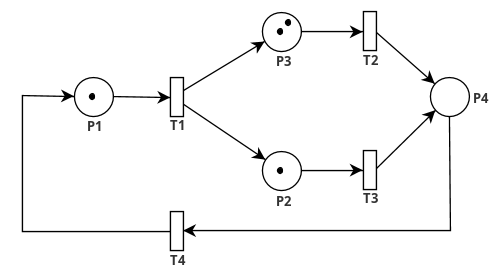
\includegraphics[width=0.6\linewidth]{images/rdp_marcada.png}
    \caption{Red de Petri marcada}
    \label{fig:rdp_marcada}
\end{figure}

\subsection{Estructura de una red de Petri ordinaria}
La estructura de una red de Petri puede definirse como una tupla de 5 elementos (5-tupla) de la siguiente manera:

\begin{equation}
    N = (P, T, I^-, I^+, M_0)
\end{equation}

Donde:
\begin{itemize}
    \item $P = \{P_1, P_2, ..., P_n\}$ es un conjunto finito y no vacío que contiene todas las plazas de la red.
    \item $T = \{T_1, T_2, ..., T_n\}$ es un conjunto finito y no vacío que contiene todas las transiciones.
    \item $I^-$ y $I^+$ son las matrcices pre y post respectivamente, cuya composición se abordará en la próxima sección.
    \item $M_0$ es el marcado inicial de la red. Definido como un vector con un elemento para cada plaza, donde $M_0[i]$ contendrá la cantidad de tokens en la plaza $i$ para el estado inicial.
\end{itemize}

Siguiendo con el ejemplo propuesto en la sección anterior \ref{fig:rdp_marcada}, se puede representar la red como $N = (P, T, I^-, I^+, M_0)$ donde:

\begin{itemize}
    \item $P = \{P_1, P_2, P_3, P_4\}$
    \item $T = \{T_1, T_2, T_3, T_4\}$
    \item $M_0 = [1, 1, 2, 0]$
\end{itemize}

A continuación se explicará la manera de obtener las matrices $I^-$ e $I^+$.

\subsection{Matriz de incidencia}
Las matrices $I^-$ e $I^+$ son las funciones de incidencia de entrada y salida de las plazas. Para el caso de la matriz $I^+$, denominada post, se tiene que cada elemento $post(P_i, T_j)$ contiene el peso asociado al arco que va desde $T_j$ hasta $P_i$. Este peso indica la cantidad de tokens que se generan en la plaza $P_i$ cuando la transición $T_j$ es disparada.\\

Por otro lado, en la matriz $I^-$, denominada pre, cada elemento $pre(P_i, T_j)$ contiene el peso asociado al arco que va desde $P_i$ hasta $T_j$ indica la cantidad de tokens que se retiran de la plaza $P_i$ cuando se dispara la transición $T_j$.\\

Siguiendo con el ejemplo de la Figura \ref{fig:rdp_marcada}, las matrices $I^-$ e $I^+$ asociadas son:
\begin{equation}
I^+ =
    \begin{pmatrix}
        0 & 0 & 0 & 1\\
        1 & 0 & 0 & 0\\
        1 & 0 & 0 & 0\\
        0 & 1 & 1 & 0
    \end{pmatrix}
\end{equation}
    
\begin{equation}
I^- =
    \begin{pmatrix}
        1 & 0 & 0 & 0\\
        0 & 1 & 0 & 0\\
        0 & 0 & 1 & 0\\
        0 & 0 & 0 & 1
    \end{pmatrix}
\end{equation}

Las filas de las matrices representan las plazas mientras que las columnas representan las transiciones, lo cual quiere decir que las matrices tendrán tantas filas como plazas tenga la red de Petri, y tantas columnas como transiciones.\\

De esta forma se puede observar como el elemento $I^-[0][0]$ indica la relación de salida entre $P_1$ y $T_1$. Más precisamente indica que cuando $T_1$ se dispara, solo un token es retirado de $P_1$ (ya que el peso del arco entre $P_1$ y $T_1$ es 1). De igual manera, el elemento $I^+[0][0] = 0$ indica que cuando la misma transición se dispara, no se genera ningún token en $P_1$ (ya que no existe ningún arco que parta de $T_1$ hacia $P_1$).\\

A partir de estas definiciones, se puede obtener la matriz de incidencia de la red. La misma está definida a continuación:\\

\begin{equation} I = I^+ -\ I^- \end{equation}

Cabe aclarar que una red de Petri puede reconstruirse completamente a partir de sus matrices $I^-$ e $I^+$, pero no así si se tiene sólo la matriz de incidencia $I$. Esto quiere decir que puede haber varias redes de Petri distintas con la misma matriz de incidencia, pero solamente una para las matrices $I^-$ e $I^+$. Sin embargo, cuando una red de Petri no tiene autobucles (presente cuando se tienen dos arcos con sentidos contrarios entre una misma plaza y transición), su matriz de incidencia determina completamente su estructura.\\

La matriz de incidencia asociada a la red de Petri de la Figura \ref{fig:rdp_marcada} será entonces:

\begin{equation}
I =
    \begin{pmatrix}
        0 & 0 & 0 & 1\\
        1 & 0 & 0 & 0\\
        1 & 0 & 0 & 0\\
        0 & 1 & 1 & 0
    \end{pmatrix}
-\ 
    \begin{pmatrix}
        1 & 0 & 0 & 0\\
        0 & 1 & 0 & 0\\
        0 & 0 & 1 & 0\\
        0 & 0 & 0 & 1
    \end{pmatrix}
=\ 
    \begin{pmatrix}
        -1 & 0 & 0 & 1\\
        1 & -1 & 0 & 0\\
        1 & 0 & -1 & 0\\
        0 & 1 & 1 & -1
    \end{pmatrix}
\end{equation}

\section{Dinámica de una red de Petri}
Se dice que una transición está sensibilizada cuando el marcado de todas las plazas entrantes a la transición es mayor o igual al peso de los arcos que las unen con dicha transición.\\

Antes de expresar la condición de sensibilizado de manera general, es necesario definir los siguientes conjuntos funciones:

\begin{itemize}
    \item $\bullet T_j$ es el conjunto compuesto por las plazas entrantes a $T_j$.
    \item $T_j \bullet$  es el conjunto compuesto por las plazas salientes de $T_j$.
    \item $\bullet \bullet P_i$ es el conjunto compuesto por las transiciones entrantes a las plazas que sensibilizan a las transiciones que le agregan tokens a $P_i$.
    \item $P_i \bullet \bullet$  es el conjunto compuesto por las transiciones entrantes a las plazas que sensibilizan a las transiciones que le quitan tokens a $P_i$.
    \item $m_k(P_i)$ es el marcado de la plaza Pi antes de disparar la transición $T_j$ .
    \item $m_{k+1}(P_i)$ es el marcado de la plaza $P_i$ después de disparar la transición $T_j$.
    \item $w_{ij}$ es el peso del arco $P_i \rightarrow T_j$.
    \item $w_{ji}$ es el peso del arco $T_j \rightarrow P_i$.
\end{itemize}

Entonces, el sensibilizado de una transición Tj está dado por:

\begin{equation}
    T_j \ est\acute{a} \ sensibilizada \ si \ \forall \ P_i \ \in \ \bullet T_j \Rightarrow m_k (P_i) > w_{ij}
\end{equation}

Esta definición de sensibilizado es solo válida cuando los arcos que conectan las plazas con $T_j$ son arcos comunes. \\
En la figura \ref{fig:rdp_sensibilizada} se resaltan las transiciones sensibilizadas del ejemplo anterior.

\begin{itemize}
    \item $T_1$, $T_2$, $T_3$ están sensibilizadas, mientras $T_4$ no está sensibilizada (ya que el marcado de $P_4$ es menor al peso del arco $P_4 \rightarrow T_4$ ).
\end{itemize}

\begin{figure}[H]
    \centering
    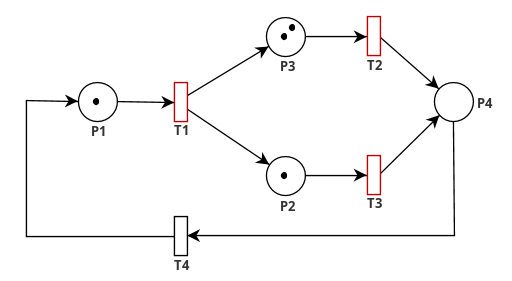
\includegraphics[width=0.6\linewidth]{images/rdp_sensibilizada.png}
    \caption{Transiciones sensibilizadas de la red de Petri}
    \label{fig:rdp_sensibilizada}
\end{figure}

\subsection{Disparo de una transición}
Si una transición está sensibilizada, la misma puede dispararse. El disparo de una transición resulta en un nuevo marcado de la red. Más precisamente, al ejecutarse una transición $T_j$ con un marcado $m_k$, los marcados de las plazas pertenecientes a la red se alteran cumpliendo con las siguientes declaraciones:

\begin{equation}
    \sigma (m_k, T_j) = 
    \begin{array}{cc}
         \forall \ P_i \ \in \ \bullet T_j \ \Rightarrow \ m_{k+1}(P_i) = m_k(P_i) - w_{ij}  \\
         \forall \ P_i \ \in \ T_j \bullet \ \Rightarrow \ m_{k+1}(P_i) = m_k(P_i) + w_{ji}  \\
         \forall \ P_i \ \notin \ \bullet T_j \cup T_j \bullet \ \Rightarrow m_{k+1}(P_i) = \ m_k(P_i)
    \end{array}
\end{equation}

\noindent Es decir:
\begin{itemize}
    \item Para todas las plazas entrantes a $T_j$, el nuevo marcado de cada plaza se habrá \textbf{decrementado} tantos $tokens$ como peso tenga el arco $P_i \rightarrow T_j$. 
    \item Para todas las plazas salientes de $T_j$, el nuevo marcado de cada plaza se habrá \textbf{incrementado} tantos $tokens$ como peso tenga el arco $T_j \rightarrow P_i$.
    \item Para el resto de las plazas, el nuevo marcado será exactamente igual al que tenían antes del disparo de $T_j$ .
\end{itemize}

Continuando con el ejemplo anterior, se puede observar en la figura \ref{fig:rdp_marcado_nuevo} el nuevo marcado de la red luego del disparo de la transición $T_3$:

\begin{itemize}
    \item La única plaza entrante a $T_3(P_3 )$, ha \textbf{decrementado} su marcado en 1 $token$ (ya que el peso del arco $P_3 \rightarrow T_3$ es 1).
    \item La plaza saliente de $T_j(P_4)$ ha \textbf{incrementado} su marcado de acuerdo a los pesos de los arcos correspondientes, en este caso en 1.
    \item Las plazas que no es entrante ni saliente de $T_3(P_3)$ ha mantenido su marcado original.
\end{itemize}

Cabe destacar que como consecuencia del disparo de $T_3$, se ha producido la sensibilización de $T_4$.

\begin{figure}[H]
    \centering
    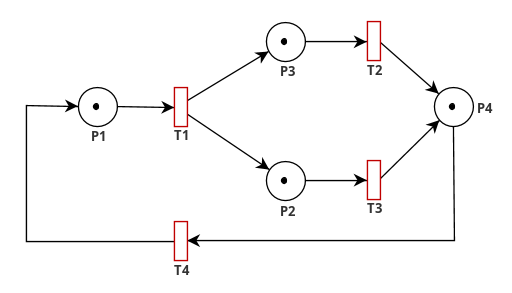
\includegraphics[width=0.6\linewidth]{images/rdp_marcado_nuevo.png}
    \caption{Nuevo marcado de la red de Petri}
    \label{fig:rdp_marcado_nuevo}
\end{figure}

\subsection{Función de transferencia y ecuación de estado}
Una vez explicada la dinámica del disparo de una transición y la forma de obtener la matriz de incidencia, se detalla una expresión matemática necesaria para obtener el nuevo marcado luego del disparo de una transición. 
La misma se denomina \textbf{función de transferencia} y está definida como el producto de la matriz de incidencia $I$ con un vector $\vec{\delta}$ cuyos componentes son todos ceros, exceptuando el componente asociado a la transición que se quiere disparar, cuyo valor será uno. Entonces, se tendrá:

\begin{equation}
    I \ . \ \vec{\delta }
\end{equation}

\noindent donde, para el disparo de una transición $T_j$ , se tiene:
\begin{itemize}
    \item $\delta[j] = 1$
    \item $\delta[i] = 0 \ \forall \ i/i \neq j$
\end{itemize}

Por otro lado, es necesario introducir la \textbf{ecuación de estado} de las redes de Petri. Con esta ecuación es posible obtener el siguiente estado del sistema luego del disparo de una transición. Esta es una manera más simple que la metodología gráfica para analizar la evolución de los sistemas. La ecuación de estado en un tiempo $i$, para calcular el nuevo marcado de la red en un tiempo $i+1$ se define como:

\begin{equation}
    M_{i+1} = M_i + I \ . \ \vec{\delta}
    \label{ec:estado}
\end{equation}

\noindent donde $M_{i+1}$ es el marcado luego del disparo de la transición, $M_i$ es el marcado antes del disparo y el segundo término de la ecuación es la función de transferencia.

Siguiendo con el ejemplo hasta ahora analizado se verá cómo calcular el marcado de la red luego del disparo de la transición $T_3$ haciendo uso de la ecuación de estado.

En la figura \ref{fig:rdp_sensibilizada} se observan las transiciones sensibilizadas de la red para el marcado inicial $M_0$.
\\
La ecuación de estado requiere tres elementos:
\begin{enumerate}
    \item El marcado antes del disparo. Éste es:
        \begin{equation}
            M_i = M_0 = 
            \begin{pmatrix}
                1 \\
                1 \\
                2 \\
                0
            \end{pmatrix}
        \end{equation}
        
    \item La matriz de incidencia de la red es la siguiente:
        \begin{equation}
           I = 
            \begin{pmatrix}
                -1 & 0 & 0 & 1 \\
                1 & -1 & 0 & 0 \\
                1 & 0 & -1 & 0 \\
                0 & 1 & 1 & -1 
            \end{pmatrix}
        \end{equation}
        
    \item El vector de disparo $\vec{\delta}$, que tendrá tantos elementos como transiciones haya en la red, cuyos valores serán cero para todas las transiciones excepto para aquella que se desee dispara:
        \begin{equation}
            \vec{\delta} = 
            \begin{pmatrix}
                0 \\
                0 \\
                1 \\
                0
            \end{pmatrix}
        \end{equation}
\end{enumerate}

\noindent con lo cual el nuevo marcado está definido por:
\begin{equation}
    M_{i+1} = 
    \begin{pmatrix}
        1 \\
        1 \\
        2 \\
        0
    \end{pmatrix}
    +
    \begin{pmatrix}
        -1 & 0 & 0 & 1 \\
        1 & -1 & 0 & 0 \\
        1 & 0 & -1 & 0 \\
        0 & 1 & 1 & -1 
    \end{pmatrix}
    .
    \begin{pmatrix}
        0 \\
        0 \\
        1 \\
        0
    \end{pmatrix}
    =
    \begin{pmatrix}
        1 \\
        1 \\
        1 \\
        1
    \end{pmatrix}    
\end{equation}

\noindent resultado que coincide con lo obtenido en la figura \ref{fig:rdp_marcado_nuevo}. La ecuación de estado representa matemáticamente el comportamiento dinámico del sistema, permitiendo calcular el nuevo estado del mismo luego de la ocurrencia de un evento a través de una simple ecuación.

\subsection{Extensión de la ecuación de estado}
Como se mencionó en la sección anterior, la ecuación \ref{ec:estado} permite calcular el siguiente estado luego del disparo de una transición. Sin embargo, puede que se desee obtener el marcado final luego de una secuencia de disparos. Suponiendo que se parte del estado inicial $M_0$, esto puede representarse como:

\begin{equation}
    M_i = M_0 + I \ . \sum_{j=1}^i u_j
\end{equation}

\noindent donde la sumatoria representa un vector asociado a la secuencia de transiciones que se desea disparar y se denomina vector S. Para ejemplificar, el cálculo de un marcado $M_i$ a partir del marcado inicial y luego del disparo de las transiciones {$T_3$, $T_4$, $T_1$, $T_2$,} está dado por:

\begin{equation}
    M_i = M_0 + I \ . \ \vec{S}
\end{equation}

\noindent donde $\vec{S}$ = \{ 1, 1, 1, 1 \} e $I$ es la matriz de incidencia asociada a la red.

\section{Propiedades de las redes de Petri}
\subsection{Propiedades de limitación}
Dada una red de Petri definida por $PN = \{ P, T, I^-, I^+, M_0 \}$, se dice que una plaza P está k-limitada si existe un número entero k que, para todo marcado posible de la red, se verifica que la cantidad de tokens de la plaza siempre es igual o menor a k. Es decir:

\begin{equation}
    \exists \ k \ \in \ N \ / \ \forall \ M \ \in \ marcados (PN) \Rightarrow M(P) \leq k
\end{equation}

\noindent Por otro lado, se dice que la red está \textbf{k-limitada} si todas las plazas que contiene son \textbf{k-limitadas}. \\ \par

A partir de la definición de limitación surgen varios conceptos, entre los cuales se encuentran los siguientes:
\begin{itemize}
    \item Una red de Petri es \textbf{segura} si todas sus plazas son \textbf{1-limitadas}. Esto significa que nunca puede darse un disparo si la plaza de llegada ya contiene un $token$.
    \item Una red de Petri es \textbf{cíclica} si siempre existe la posibilidad de alcanzar el marcado inicial desde cualquier otro marcado alcanzable. Es decir, \break $\forall \ M  \in \ marcados(PN),\ M_0$ es dinámicamente alcanzable desde $M$.
    \item Una red de Petri es \textbf{repetitiva} si existe una secuencia de disparos $\sigma$ que contiene todas las transiciones de la red y existe un marcado $M$ que para el cual $M \xrightarrow{\sigma} M$. Es decir, existe una secuencia de disparos que contiene todas las transiciones y que lleva la red del marcado actual al mismo marcado.
    \item  Una red de Petri es \textbf{conservativa} si se cumple que $\forall \ M\ \in marcados (PN)$, el número total de $tokens$ en el marcado M es igual al número de tokens en el marcado $M_0$. En otras palabras, la red siempre contiene la misma cantidad de marcas.
    
\end{itemize}

\subsection{Propiedades de vivacidad}
La \textbf{vivacidad} de una transición indica que, en todo instante de la  evolución de la red, su disparo es posible. Este concepto es particularmente relevante ya que determina si la ejecución de la red puede  o no detenerse en un estado determinado. A partir de esto se puede definir la vivacidad de una red de Petri. Esta propiedad indica que una red $N = \{P, T, I^- , I^+ , M_0 \}$ es viva para un marcado si todas sus transiciones lo son.

Por otro lado, la \textbf{cuasi-vivacidad} de una transición expresa la posibilidad de dispararla al menos una vez a partir de un marcado inicial $M_0$. De la misma manera que para el caso de la vivacidad, una red de Petri es cuasi-viva si todas sus transiciones lo son.

Gracias a esta última definición, se puede definir la vivacidad en función de la cuasi-vivacidad de la siguiente manera: una transición es viva si la misma es cuasi-viva en la red para todo marcado alcanzable desde $M_0$. \\ \par

\noindent La vivacidad está directamente asociada con la ausencia de \textbf{deadlock} o interbloqueo. En términos generales, el deadlock es el bloqueo permanente de un conjunto de procesos o hilos de ejecución en un sistema concurrente que compiten por recursos del sistema o bien se comunican entre ellos. En el caso de una red de Petri, esto suele ocurrir cuando dos o más transiciones esperan mutuamente por el disparo de la otra, produciendo el bloqueo permanente de esa porción de la red. 
Una red de Petri viva garantiza la ausencia de interbloqueo sin importar la secuencia de disparos.

\subsection{Alcanzabilidad de una red de Petri}
La \textbf{alcanzabilidad} de una red de Petri es fundamental para el análisis de las propiedades dinámicas de un sistema. A grandes rasgos, permite determinar si el sistema modelado puede alcanzar un determinado estado.

Un marcado $M_i$ es alcanzable desde $M_0$ si existe una secuencia finita de disparos $\sigma$ tal que $M_0 \xrightarrow{\sigma} M_i$.

Los marcados alcanzables por la red pueden ser representados como nodos de un grafo o árbol, donde los arcos indican los disparos necesarios para alcanzar dicho marcado. El algoritmo para determinar el árbol de alcanzabilidad de una red de Petri será explicado con detalle en el desarrollo del proyecto.

Entonces, el grafo de alcanzabilidad $A$ se define como el menor conjunto que cumpla con las expresiones \ref{ec:marcado_inicial} y \ref{ec:marcado_alcanzable}.

\begin{equation}
    M_0 \ \in \ A
    \label{ec:marcado_inicial}
\end{equation}

\noindent Esta condición simplemente aclara que el marcado inicial de la red siempre forma parte del grafo de alcanzabilidad, ya que el mismo no requiere ninguna secuencia de disparos para ser alcanzable.

\begin{equation}
    \forall \ M \ sii \ M \xrightarrow{\sigma} M_i \Rightarrow M_i \ \in \ A
    \label{ec:marcado_alcanzable}
\end{equation}

\noindent Esto significa que para cualquier marcado $M$, si a partir del mismo puede alcanzarse otro marcado $M_i$, entonces $M_i$ forma parte del grafo. \\ \par

\noindent Suponiendo una red simple como la de la figura \ref{fig:rdp_3_estados}, compuesta por tres plazas y una única transición $T_1$ , se puede afirmar que sólo hay tres estados posibles en la red:

\begin{figure}[H]
    \centering
    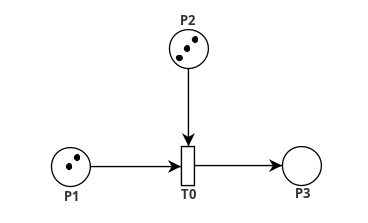
\includegraphics[width=0.5\linewidth]{images/rdp_3_estados.png}
    \caption{Red de Petri 3 estados posibles}
    \label{fig:rdp_3_estados}
\end{figure}

\begin{itemize}
    \item El marcado inicial [2, 3, 0]
\end{itemize}

Luego del segundo disparo no existen disparos posibles. Por lo tanto, la red de la figura \ref{fig:rdp_3_estados} produce el grafo de alcanzabilidad mostrado en la figura \ref{fig:grafo_alcanzabilidad}. \\

\begin{figure}[H]
    \centering
    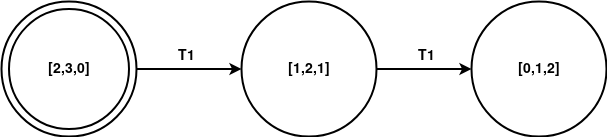
\includegraphics[scale=0.4]{images/grafo_alcanzabilidad.png}
    \caption{Grafo de alcanzabilidad.}
    \label{fig:grafo_alcanzabilidad}
\end{figure}

\subsection{Sifones y Trampas}
Los conceptos de sifón y trampa están directamente relacionados con las propiedades de \textbf{interbloqueo} y \textbf{vivacidad} de una red de Petri.

Un \textbf{sifón} se define como un subconjunto no vacío de plazas S para el cual se cumple que el subconjunto de transiciones entrantes a S está contenido dentro del subconjunto de transiciones salientes de S.
En otras palabras, un grupo de plazas es un sifón si, una vez que un token sale del grupo de dichas plazas, el mismo nunca puede volver a entrar. 
Decimos que un sifón S es \textbf{mínimo} si no contiene otro sifón como un subconjunto. En un sifón mínimo debe existir al menos dos lugares; de lo contrario, la estructura restante no puede considerarse un sifón.
En la figura \ref{fig:rdp_sifon_trampa} se puede observar una red que contiene una trampa y un sifón.

\begin{figure}[H]
    \centering
    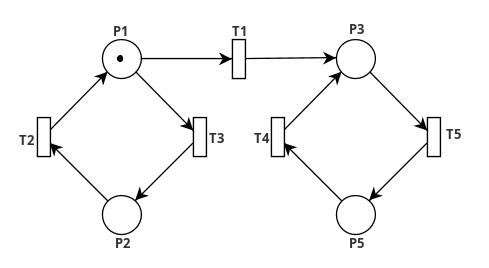
\includegraphics[width=0.8\linewidth]{images/rdp_sifon_trampa.png}
    \caption{Sifón y trampa}
    \label{fig:rdp_sifon_trampa}
\end{figure}

Tomando el subconjunto de plazas $S = \{P_1 , P_2 \}$ se deben obtener los siguientes subconjuntos de transiciones:
\begin{itemize}
    \item El subconjunto $\bullet S = \{T_2, T_3 \}$ será aquel compuesto por las transiciones entrantes a las plazas que componen S.
    \item El subconjunto $S \bullet = \{T_2, T_3\} $ será aquel compuesto por las transiciones entrantes a las plazas que componen S.
\end{itemize}

\noindent Por propiedad de los sifones, para que S pueda considerarse como tal debe cumplirse que:
\begin{equation}
    \bullet S \ \subseteq \ S \bullet 
\end{equation}

En este caso, se comprueba que ${T_2 , T_3} \subseteq \ \{T_1 , T_2 , T_3 \}$, quedando demostrado que $\{P_1,P_2\}$ es en efecto un sifón y que, si la transición $T_1$ se dispara, el token removido de $P_1$ nunca volverá a ingresar al subconjunto. \\ \par

Por otro lado, una \textbf{trampa} se define como un subconjunto de plazas G para el cual se cumple que el subconjunto de transiciones salientes de G está contenido dentro del subconjunto de transiciones entrantes a G. Esto quiere decir que un conjunto de plazas constituyen una trampa si una vez que un token entra dicho grupo éste nunca vuelve
a salir.

Siguiendo con el ejemplo de la figura \ref{fig:rdp_sifon_trampa}, se analizará el subconjunto de plazas $G = \{P_3 , P_4\}$.  Los subconjuntos de transiciones serán:
\begin{itemize}
    \item El subconjunto $\bullet G = \{T_1 , T_4 , T_5 \}$ será aquél compuesto por las transiciones entrantes a las plazas que componen G.
    \item El subconjunto $G \bullet = \{T_4, T_5 \}$ será aquél compuesto por las transiciones salientes de las plazas que componen G.
\end{itemize}

\noindent Por propiedad de las trampas, para que G pueda considerarse como tal, debe cumplirse que:
\begin{equation}
    G \bullet \ \subseteq \ \bullet G
\end{equation}

Propiedad que es simplemente comprobable ya que ${T_4 , T_5} \subseteq \{T_1 , T_4 , T_5 \}$, demostrando que $\{P_3 , P_4\}$ es una trampa.

\subsection{Invariantes de plazas y transiciones}
Las invariantes de una red son propiedades independientes tanto del marcado inicial como de la secuencia de disparos, y pueden asociarse a ciertos subconjuntos de plazas o de transiciones; con lo cual surgen dos conceptos:

\subsubsection{P-invariantes}
Una \textbf{invariante de plazas} o \textbf{P–invariante} es un conjunto de plazas cuya suma de tokens no se modifica con una secuencia de disparos arbitraria. 
Esto se puede observar en el ejemplo de la figura \ref{fig:rdp_p_invariantes}:

\begin{figure}[H]
    \centering
    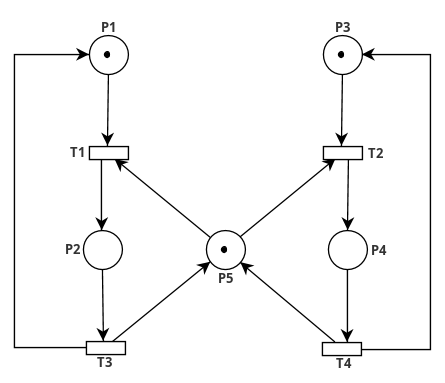
\includegraphics[width=0.7\linewidth]{images/rdp_p_invariantes.png}
    \caption{P-invariantes de la red de Petri}
    \label{fig:rdp_p_invariantes}
\end{figure}

\noindent Tras el análisis de la red , se obtienen las siguientes invariantes de plazas:
 
\begin{equation}
   \begin{array}{cc}
       m(P_1) + m(P_2) = 1  \\
       m(P_3) + m(P_4) = 1   \\
       m(P_2) + m(P_4) + m(P_5) = 1 
   \end{array}
\end{equation}

El primer ítem expresa que la sumatoria de tokens en las plazas $P_1$ y $P_2$ siempre será igual a uno, afirmación completamente observable al mirar la red de la figura \ref{fig:rdp_p_invariantes}. Estas declaraciones implican la siguiente consecuencia:

\begin{equation}
   I . x = 0
\end{equation}

\noindent donde $I$ es la matriz de incidencia y $x$ es un vector característico de un subconjunto $Q$ de las plazas que forman parte de la invariante (un uno en una posición indica que esa plaza es parte de la invariante y un cero indica lo contrario). A partir de esto surge la siguiente fórmula:

\begin{equation}
    \sum_{P \in \bullet t \cap Q} W(p,t) = \sum_{P \in t \bullet \cap Q} W(t,p)
\end{equation}

\noindent la cual puede ser expresada en función de un vector t de la siguiente manera:

\begin{equation}
    \sum_{P \in \bullet t \cap Q} t(p) = \sum_{P \in t \bullet \cap Q} t(p)
\end{equation}

\noindent Esto quiere decir que:

\begin{equation}
    \sum_{P \in (t \bullet \cup \bullet t) \cap Q} t(p) = 0 \ \ y \  \sum_{P \in Q} t(p) = 0
\end{equation}

Si reemplazamos $Q$ por los vectores característicos $I_q$ , estas dos igualdades pueden escribirse como:

\begin{equation}
    \sum_{P \in Q} t(p) I_q(p) = 0 \ \ y \  \sum_{p \in P} t(p)I(p) = 0
\end{equation}

\noindent Lo cual es simplemente la definición del producto escalar entre dos vectores:

\begin{equation}
    t.I_q = 0
\end{equation}

\noindent Como los disparos son arbitrarios, podemos establecer la siguiente relación:
\begin{equation}
    t_j I_q; \forall \ t_j \ \in \ T \Longleftrightarrow \ I^T I_q = 0
\end{equation}

\noindent donde $I^T$ es la matriz de incidencia transpuesta.

\subsubsection{T-invariantes}
Un \textbf{invariante de transición} ó \textbf{T-invariante} es el conjunto de transiciones que deben dispararse para que la red de Petri retorne a su estado inicial.

Como se mencionó en el apartado anterior, para el cálculo de las P-invariantes se hace uso de la ecuación $I . x = 0$, siendo $I$ la matriz de incidencia y $x$ un vector característico constituido por las plazas que forman parte de la invariante. En este caso, para el cálculo de los vectores que constituyen las T-invariantes, la ecuación asociada será similar a las P-invariantes, a diferencia que se hace uso de  $I^T$ en vez de $I$:

\begin{equation}
    I^T . x = 0
\end{equation}

Aquí, a diferencia de las P-invariantes, el vector x está constituido por el conjunto de transiciones que deben dispararse para que la red retorne al estado inicial. Un "1" en una posición indica que esa transición es parte de la invariante y un "0" indica lo contrario.

Tomando la figura \ref{fig:rdp_p_invariantes} como ejemplo y se obtienen las siguientes invariantes de transiciones:

\begin{equation}
    T-invariantes = 
    \begin{pmatrix}
         T0 & T1 & T2 & T3  \\
         0 & 1 & 0 & 1  \\
         1 & 0 & 1 & 0  
    \end{pmatrix}
\end{equation}

Ambos vectores cumplen la condición planteada ($I^T .\ x = 0$) y si se observa la imagen en cuestión, se puede apreciar que la red retorna a su estado inicial si las transiciones especificadas en los vectores se disparan.

\section{Concurrencia y sincronización}
En los sistemas de computación actuales conviven múltiples procesos que cooperan para lograr determinados objetivos y compiten por recursos del sistema, entre ellos el procesador, la memoria RAM, los puertos de entrada/salida, etc.\\
Dado que generalmente el numero de procesos de un sistema supera ampliamente el numero de recursos, se deben establecer formas de comunicación y sincronización entre ellos que hagan que el sistema funcione correctamente. 

\par En ésta sección se definirá cuando dos programa son concurrentes y/o paralelos y las condiciones que deben cumplirse para que dos secciones de código fuente puedan ser ejecutadas de manera concurrente. Luego, se verá que la ejecución concurrente de procesos trae aparejados ciertos problemas como el interbloqueo y la inanición.\\
Por esta razón deben ejecutarse ciertos mecanismos de control para garantizar la correcta ejecución de los programas, entre ellos, los semáforos y monitores.\\
El objetivo de esta sección es que el lector adquiera una idea general sobre la programación concurrente y sobre los problemas inherentes a la misma.

\subsection{Concurrencia y paralelismo}
Dos procesos serán concurrentes cuando la primera instrucción de uno de ellos se ejecuta después de la primera instrucción de otro proceso y antes de la última.
No es necesario que estos se ejecuten al mismo tiempo, basta con el hecho de que se intercalen sus instrucciones. En caso de ejecutarse al mismo tiempo se dice que hay programación paralela.
La programación concurrente es un paralelismo potencial, dependiente del hardware que lo soporte  \cite{mendez}.

\subsubsection{Problemas inherentes a la programación concurrente}
La intercalación de instrucciones de diferentes procesos, debe ser bien manejada y controlada dado que puede producir mal funcionamiento del sistema. Los problemas inherentes a la concurrencia son:
\begin{itemize}
    \item \textbf{Exclusión mutua}: Se debe garantizar que si un proceso adquiere el recurso los demás deberán esperar hasta que sea liberado.

    \item \textbf{Condición de sincronización}: Hay situaciones en las que un proceso debe esperar que ocurra algún determinado evento para poder continuar. Por ello se debe garantizar que si el evento \textbf{no} ocurrió, el proceso \textbf{no} continúe. 
    
    \item \textbf{Interbloqueo}: Esta situación se produce cuando todos los procesos están esperando un evento que nunca ocurrirá. Se debe garantizar que estas situaciones no ocurran.
    
    \item \textbf{Inanición}: En este caso, el sistema en su conjunto hace progresos, pero existe un grupo de procesos que nunca progresaran pues no se les otorga tiempo de procesador para hacerlo.
\end{itemize}

\subsubsection{Exclusión mutua}
La exclusión mutua implica que dos o más procesos intentan acceder a un único recurso compartido entre ellos pero solo uno puede acceder a cada instante.
Cuando se da un caso de estas características, se desea que todo lo que necesite hacer unos de los procesos sobre el recurso se realice de manera indivisible y luego lo deje disponible para que otro proceso ejecute sus instrucciones sobre el recurso.
\par A la porción de código que se desea que se ejecute de manera indivisible o atómica se le llama \textbf{sección crítica}. Se debe lograr que todas las instrucciones dentro de la sección crítica se ejecuten en exclusión mutua lo que implica que el hecho de que cuando uno de los procesos este ejecutando esa porción de código el resto no podrá hacerlo. \\
\\
\textbf{Solo uno de los procesos podrá estar en la sección crítica en un instante dado.}

\begin{figure}[H]
    \centering
    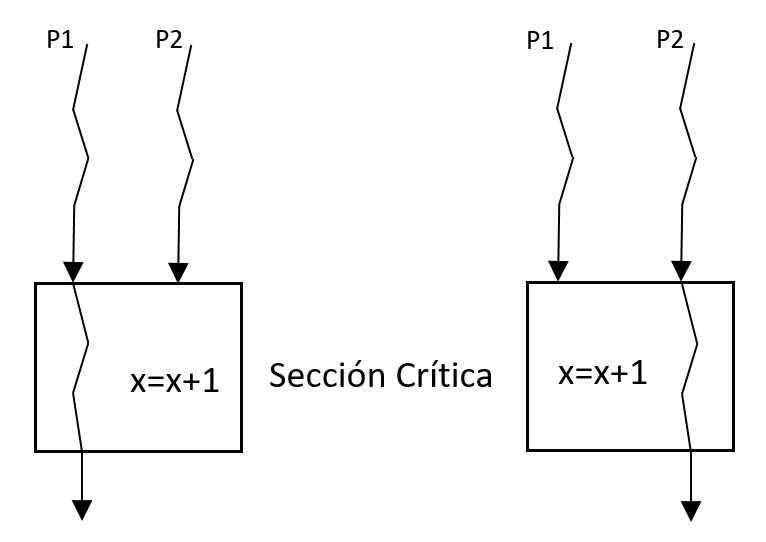
\includegraphics[scale=0.4]{images/seccion_critica.jpg}
    \caption{Sección crítica}
    \label{fig:seccion_critica}
\end{figure}

En la figura \ref{fig:seccion_critica} se observa como dos procesos $P1$ y $P2$ intentan ejecutar una porción de código de una sección crítica. La imagen de la izquierda (a) muestra que el proceso $P1$ consigue ingresar a ejecutar la sección crítica. La imagen de la derecha (b) muestra que el proceso $P2$ puede ingresar solo cuando el proceso $P1$ ya no esta en la misma.

\noindent La exclusión mutua se puede representar de la siguiente manera.
\begin{figure}[H]
    \centering
    \includegraphics[scale=0.7]{images/rdp_seccion_crítica.png}
    \caption{Sección crítica}
    \label{fig:rdp_seccion_crítica}
  \end{figure}

En la figura \ref{fig:rdp_seccion_crítica} la plaza \textit{MUTEX} esta limitada a un único token y el análisis de invariantes de plazas demuestra formalmente la propiedad de exclusión mutua entre los procesos $P1$ y $P2$. 

\begin{equation}
    m(EjecutandoSCP1) + m(MUTEX) + m(EjecutandoSCP2) = 1
\end{equation}

\subsection{Interbloqueo}
En un sistema donde los procesos compiten por limitados recursos, pueden producirse demandas contradictorias de los mismos. Por ejemplo, si existen dos procesos, \textit{A} y \textit{B}, y dos recursos \textit{R1} y \textit{R2}, y ambos procesos necesitan los dos recursos para proseguir, si el proceso \textit{A} toma el recurso \textit{R1} y el \textit{B} el recurso \textit{R2}, ambos procesos se bloquearan a la espera del otro recurso, pero ninguno liberará el recurso que posee hasta no conseguir los dos. A esta situación se la conoce como interbloqueo. 

\subsubsection{Condiciones para producir interbloqueo: }
\noindent Deben presentarse tres condiciones de gestión para que sea posible un interbloqueo:
\begin{enumerate}
    \item \textit{Exclusión mutua}: sólo un proceso puede utilizar un recurso en cada momento. Ningún proceso puede acceder a un recurso que se ha asignado a otro proceso.
    
    \item \textit{Retención y espera}: un proceso puede mantener los recursos asignados mientras espera la asignación de otros recursos.
    
    \item \textit{No apropiación}: ningún proceso podrá ser forzado a abandonar un recurso que retiene.
    
    \item \textit{Espera circular}: existe una cadena cerrada de procesos donde cada proceso retiene un recurso que necesita un proceso que le sigue en la cadena.
\end{enumerate}

Las tres primeras condiciones son necesarias pero no suficientes para que exista interbloqueo.
La cuarta es una consecuencia potencial de las tres primeras y, en caso de darse, generará una \textbf{espera circular irresoluble}. Esta es de hecho la definición de interbloqueo.

\subsection{Sincronización}
Para solucionar los problemas inherentes a la programación concurrente, se utiliza lo que se llama \textit{sincronización entre los procesos} . \\
Se habla de sincronización , en general, cuando determinados fenómenos ocurren o deben ocurrir en un determinado orden o a la vez.
\par Para la computación, la sincronización es representada por las señales que se envían los procesos para colaborar entre ellos o para indicar el estado de recursos compartidos, para indicar que un evento o acción ocurrió o no y determinar la continuidad o no de un proceso, etcétera.
\par La condición de sincronización puede definirse como la propiedad requerida para que un proceso no realice ninguna acción o evento hasta que otro proceso realice una determinada acción o evento.

\subsubsection{Semáforos}
Los semáforos son un sistema de señales simples utilizadas por los procesos para comunicarse entre ellos y lograr la sincronización requerida.
Estos tienen una variable de sincronización, del tipo entero no negativo, que indica la cantidad de recursos disponibles. Sobre esta se realizan dos tipos de operaciones:

\begin{itemize}
    \item \textit{wait}: decrementa el valor del semáforo solo si este es mayor que cero. Este proceso indica que se utiliza uno de los recursos que controla el semáforo. Si el valor del semáforo al momento de ejecutar la operación \textit{wait} es cero, indica que no hay recursos disponibles y el proceso deben bloquearse hasta que se libere alguno.
    \item \textit{signal}: es la acción de liberar un recurso que estaba siendo utilizado. En caso de haber algún proceso bloqueado en el semáforo se lo despierta para que utilice el recurso. De no existir algún proceso, se incrementa el valor del semáforo.
\end{itemize}

Los semáforos son primitivas con las cuales es difícil expresar una solución a grandes problemas de concurrencia, ya que tienen algunas debilidades:
\begin{itemize}
    \item La omisión de una de las primitivas puede corromper el funcionamiento de un sistema concurrente.
    \item El control de concurrencia es responsabilidad del programador.
    \item Las primitivas de control se encuentran esparcidas por todo el código, lo que hace muy difícil la corrección de errores y el mantenimiento del mismo.
\end{itemize}

Debido a estas razones existe otro mecanismo de software para el control de concurrencia denominado \textbf{monitor}.

\subsubsection{Monitores}
Como se dijo, los semáforos, generalmente se encuentran dispersos en el código, lo que lo hace más confuso y muchas veces es difícil notar cual es el recurso compartido y determinar si está correctamente sincronizado. Por ello, se necesita un sistema que sea igual de versátil que los semáforos pero que permita efectuar un control más estructurado de la exclusión mutua. Una herramienta con estas características fue propuesta por \textit{C.A.R Hoare} en 1975 y es conocida como \textbf{\textit{monitor}}.\\
Un \textbf{monitor} es un mecanismo de abstracción de datos, lo que permite representar de forma abstracta un recurso compartido mediante variables que indican su estado. El acceso a esas variables solo es posible a través de un conjunto de funciones/métodos que el monitor exporta al exterior.\\

Un monitor se compone de los siguientes elementos:
\begin{itemize}
    \item Un \textit{conjunto de variables} locales que pueden denominarse permanentes. Se utilizan para almacenar el estado interno del recurso que representa el monitor. Se denominan permanentes ya que permanecen sin modificarse entre dos llamadas consecutivas al monitor y solo pueden ser accedidas dentro del mismo.
    
    \item Un \textit{código de inicialización} que se ejecuta antes que la primera instrucción ejecutable del programa y su fin es inicializar las variables permanentes. 

    \item Un \textit{conjunto de procedimientos internos} que manipulan las variables permanentes.
    
    \item Una \textit{declaración de los procedimientos} que son \textit{exportados} y pueden ser accedidos por los procesos activos externos.
\end{itemize}

\paragraph{Exclusión mutua en monitores}
\hfill
\par El control de la exclusión mutua en un monitor se basa en la existencia de una cola asociada al mismo que se denominara \textit{cola del monitor}. La gestión de esta cola se realiza de la siguiente manera:

\begin{enumerate}
    \item Cuando un proceso activo está dentro del monitor (ejecutando alguno de los procedimientos del mismo) y aparece otro proceso activo que intenta ejecutar otro (o el mismo) procedimiento, el código de acceso al monitor bloquea el proceso que realiza la llamada y lo inserta en la cola del monitor (con política FIFO). Así, se impide que dos procesos estén al mismo tiempo dentro del monitor.

    \item Cuando un proceso activo abandona el monitor, este ultimo selecciona el proceso que esta al frente de la cola del monitor y lo desbloquea para que comience a ejecutar las operaciones que le solicitó al monitor. Si la cola estaba vacía, el monitor queda libre y cualquier proceso activo que llame alguno de sus procedimientos entrará al monitor.
\end{enumerate}

Esto asegura que las variables compartidas nunca son accedidas concurrentemente. Una cuestión importante es que la responsabilidad de bloquear un proceso es del monitor y no del proceso.
Al comparar este sistema con un semáforo se ve que en el caso de los semáforos son los propios procesos activos los que manejan las políticas de acceso a variables compartidas.

\paragraph{Condición de sincronización en monitores}
\hfill
\par El procedimiento anterior sólo controla la exclusión mutua, es decir, pueden haber casos donde un proceso activo tenga acceso al monitor (ha obtenido la exclusión mutua al mismo) pero no puede seguir su ejecución debido a alguna razón, tal como un \textit{buffer} lleno que no puede ser escrito. En estos casos, es necesario bloquear ese proceso y permitir que otro ingrese al monitor. Para realizar esto surgen nuevos componentes que deben formar parte del monitor:

\begin{itemize}
    \item Variables de condición
    \begin{itemize}
        \item Las mismas son declaradas en el monitor. 
        \item Deben ser privadas. 
        \item Tienen una cola \textit{FIFO} asociada.
    \end{itemize}
    \item Operaciones sobre las variables de condición
    \begin{itemize}
        \item \textit{Delay}
        \item \textit{Resume}
        \item \textit{Empty}
    \end{itemize}
\end{itemize}

La operación delay se realiza sobre una variable de condición. Si se supone la existencia de una variable C, al realizar \textit{delay(C)}, el proceso que la ejecutó libera el mutex del monitor, se bloquea y se envía al final de la cola asociada a la condición C. A diferencia de la operación wait que se utiliza en los semáforos, delay bloquea al proceso incondicionalmente.\\

\par La operación resume, cuando se realiza sobre una variable C, libera al primer proceso que ejecutó \textit{delay(C)}. Si la cola está vacía, resume es una operación nula. Por otra parte, la función empty simplemente devuelve un valor boolean true si una cola se encuentra vacía o false en caso contrario.\\

Con lo dicho hasta este punto, se podría decir que si un proceso que se está ejecutando dentro del monitor ejecuta una operación \textit{resume(C)}, se desbloqueará un proceso de esa cola que continuará con su ejecución dentro del monitor también. Esto lleva a una situación con dos procesos dentro del monitor, lo que violaría la exclusión mutua. Para evitar esto, el proceso que ejecuta el \textit{resume} cederá la exclusión mutua al recien desbloqueado. Y espera en una cola diferente llamada \textbf{cola de cortesía} hasta que el proceso recién desbloqueado por el \textit{resume(C)} termine su ejecución teniendo preferencia por sobre los procesos esperando en otras colas.

\begin{figure}[H]
    \centering
    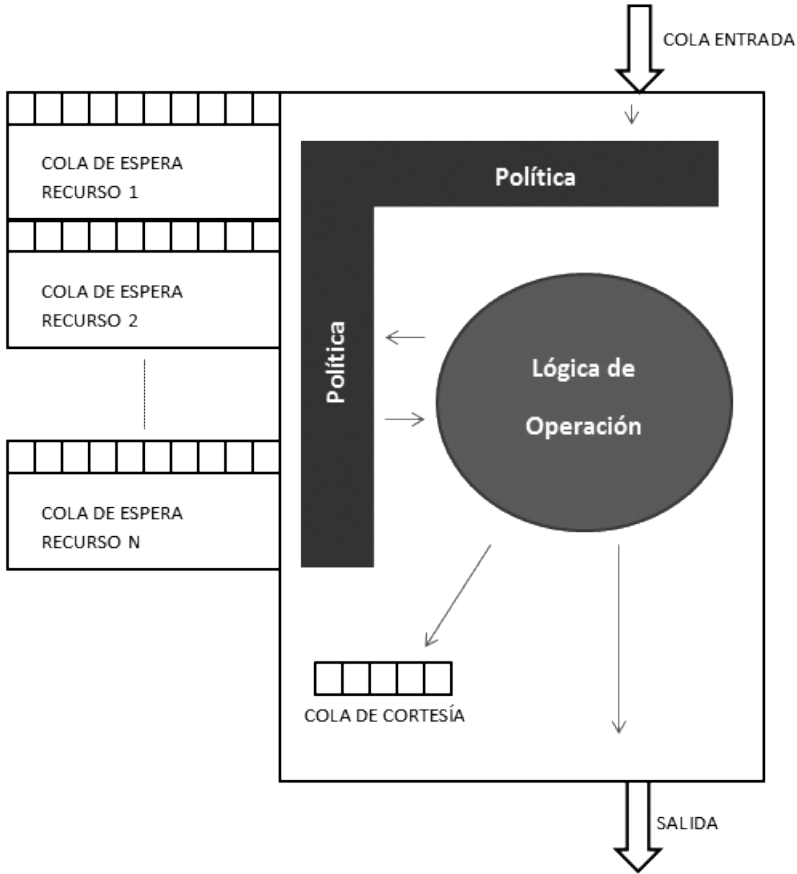
\includegraphics[scale=0.5]{images/monitor_mico.png}
    \caption[Monitor.]{Figura adaptada del Proyecto Integrador \textit{Desarrollo de IP cores con procesamiento de Redes de Petri Temporales para sistemas multicore en FPGA}}
    \label{fig:monitormico}
\end{figure}

\subsubsection{Implementación de monitores con redes de Petri}
Es posible ver a un monitor formado por dos secciones: primero, la referida a la política de colas que se debe ejecutar para lograr que sólo un proceso esté en el monitor, que se bloqueen los procesos que no tienen los recursos y que se desbloqueen los que obtuvieron los recursos, y segundo, la lógica con que se administran los recursos.\\
En la figura \ref{fig:monitormico} se puede observar que existe una cola de entrada, para los procesos que aún no ingresaron al monitor y desean hacerlo, una serie de colas, una por cada recurso (cada condición de sincronización) y una cola de cortesía para que  proceso dentro del monitor pueda, de manera segura, ceder la exclusión mutua al cambiar el estado de un recurso.\\

\par \textbf{\textit{Una red de Petri puede realizar el trabajo de la lógica del monitor}}, es decir, la administración y sincronización de recursos disponibles; esto es cuando el vector de estado que resultó del disparo no tiene componentes negativas es porque los recursos están disponibles, el disparo de la transición solicitada conduce a un nuevo estado valido. De no ser así, en caso de existir algún valor negativo en el nuevo vector de estado, se llegó a un estado no válido que indica que el recurso no está disponible. Además el vector de estado indica si el disparo ha devuelto o tomado recursos. Si la cantidad de tokens para un recurso dado disminuye, significa que se han tomado recursos, en caso contrario, que se han devuelto recursos.

\begin{figure}[H]
    \centering
    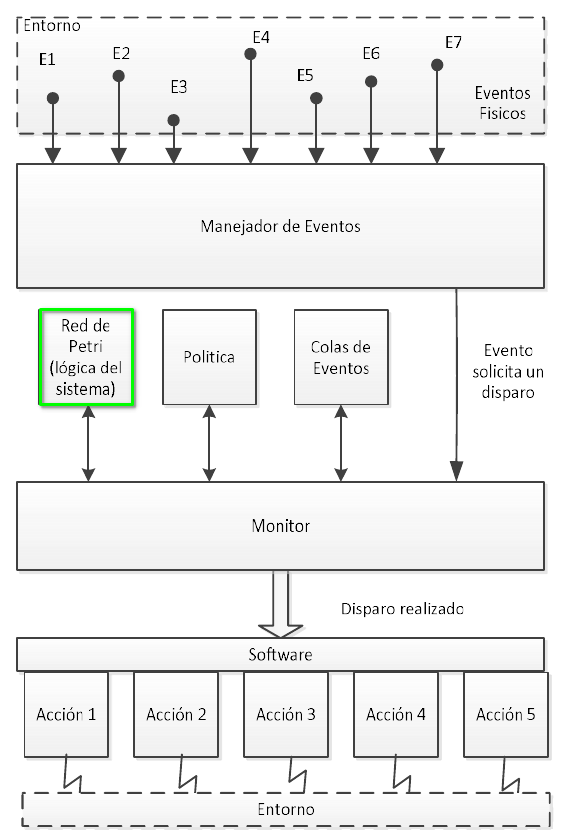
\includegraphics[scale=0.5]{images/monitor_mico_1.png}
    \caption[Monitor.]{Monitor figura adaptada del paper publicado por \textit{Micolini, Orlando \& Ventre, Luis \& Cebollada, Marcelo \& Eschoyez, Maximiliano}}
    \label{fig:monitormico1}
\end{figure}

Por lo tanto, el monitor integra la red de Petri (lógica), la política y las acciones, conformando un sistema heterogéneo. La importancia de la metodología aquí planteada radica en desacoplar la lógica de la política y las acciones, con el fin de obtener un sistema resultante modular, simple, mantenible y verificable. 

En la figura \ref{fig:monitormico1} se expone la arquitectura modular de un sistema reactivo y guiado por eventos.
